\chapter[Desenvolvimento]{Desenvolvimento}
\label{ch:desenvolvimento}
O \textit{Power Monitor} surgiu da necessidade da conscientização do gasto energético e da melhor compreensão da conta de luz. Baseado nesse conceito,
foram desenvolvido um \textit{software} que permitirá uma fácil comunicação com qualquer equipamento construído que tenha a finalidade de monitorar a energia elétrica e um \textit{hardware} para demonstração
da comunicação entre ambos. O sistema traz uma forma mais fácil e próxima do consumidor final de se quantificar a energia elétrica consumida em um estabelecimento. No lugar do Quilowatt-hora, medida que é usada atualmente,
o \textit{software} propõe mensurar o gasto energético em reais (R\$), trazendo a realidade do consumo mensal para mais próximo de cada brasileiro.

Nesse capítulo será mostrado todo o passo a passo para o desenvolvimento do \textit{software} e \textit{hardware}, juntamente com a comunicação 
entre ambos, por fim será mostrado os resultados obtidos. Em resumo pode-se ter uma visão geral de como o ambiente - \textit{software} e 
\textit{hardware} - funciona observando a \autoref{fig:diagrama-vg} e para complemento da informação, a Y mostra o driagama de ações do ambiente.

\begin{figure}[h!]
	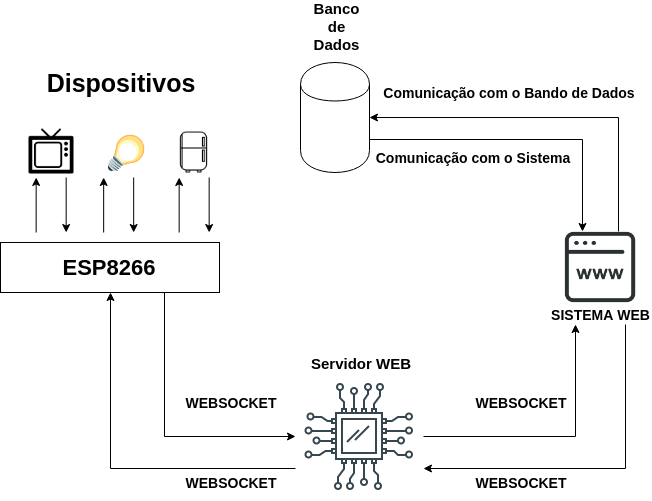
\includegraphics[width=0.7\textwidth, keepaspectratio=true]{diagrama-1}
	\centering
	\caption[Visão geral do ambiente]{Visão geral do ambiente}
	\label{fig:diagrama-vg}
\end{figure}
\FloatBarrier

\section[\textit{Software}]{\textit{Software}}\label{soft-sec}
O controle dos dispositivos de um cômodo que estão interligado com o \textit{hardware}ou casa são controlados pelo \textit{software}. Dessa forma
todos os dispositivos que estão interligados ao microcontrolador e que estão cadastrados nos sistema podem ser controlados (Ligar/Desligar) e também
é possível o acompanhamento dos gastos.

O sistema possui uma interface \textit{web} que pode ser acessada por qualquer dispositivo que tenha acesso a internet e possua um 
\textit{browser}.O \textit{software} possui uma interface de apenas um único usuário, ao acessar o sistema o usuário se depara com um
visual bem agradável e fácil de se usar. Ao entrar no sistema o usuário se depara com a página principal, \autoref{fig:principal-ft}, nela se encontram
as principais informações que o usuário irá precisar, como também mostra as oções de cadatrar novo dispositivo, listar os dispositivos, cadastrar novo cômodo,
listar um novo cômodo etc.

\begin{figure}[h!]
	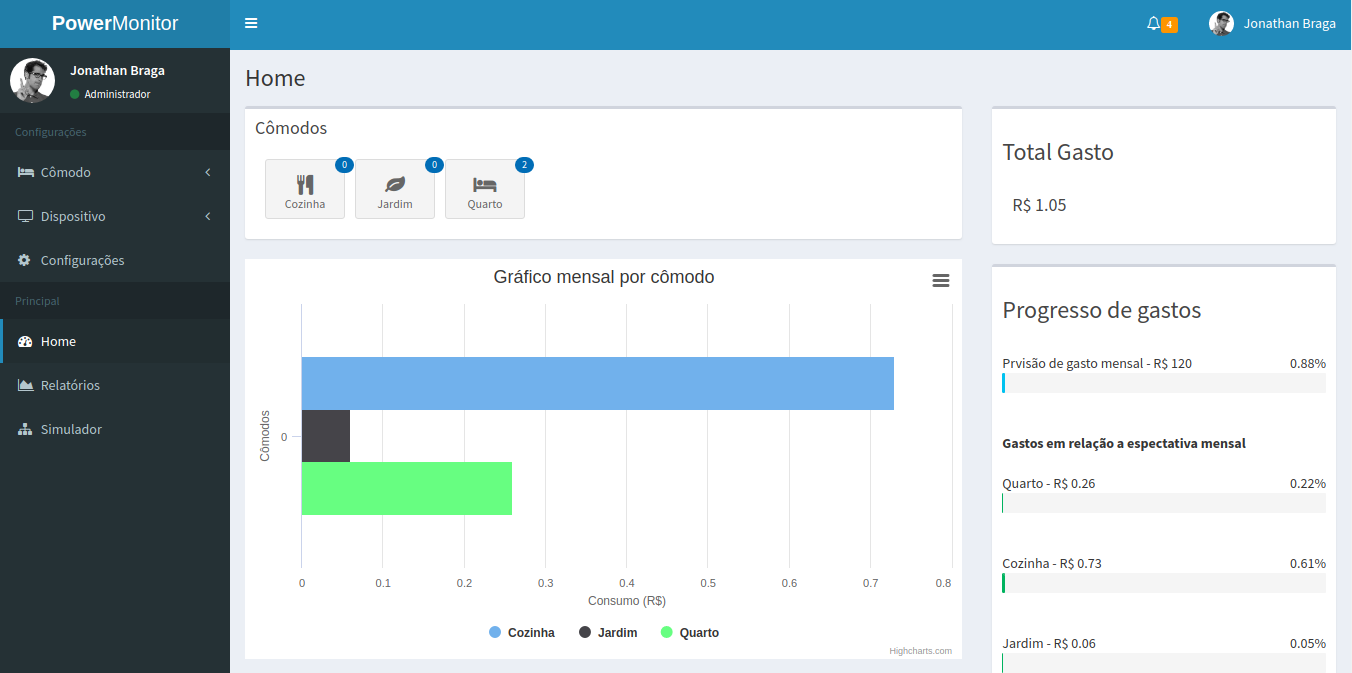
\includegraphics[width=1.0\textwidth, keepaspectratio=true]{principal}
	\centering
	\caption[Tela inicial do sistema]{Tela inicial do sistema}
	\label{fig:principal-ft}
\end{figure}
\FloatBarrier


\section[\textit{Hardware}]{\textit{Hardware}}\label{hard-sec}
\section[\textit{Resultados}]{\textit{Resultados}}\label{resultados-sec}
